\subsubsubsubsection{Parking manager}
\begin{figure}[h]
\centering
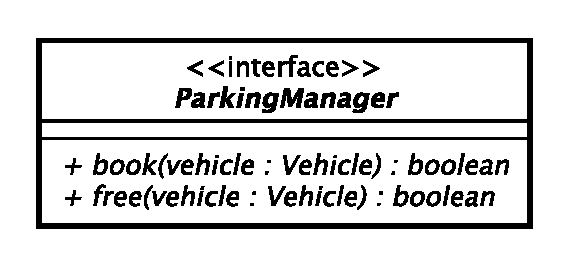
\includegraphics[scale=0.6,keepaspectratio]{images/solution/app/backend/parking_manager.eps}
\caption{\pReactiveComponentStretchDecoration::ParkingManager}
\label{fig:sd-app-parking-manager}
\end{figure}
\FloatBarrier
\begin{itemize}
  \item \textbf{\descr} \\
    It represents an entity that manages a parking lot.
  \item \textbf{\ops}
  \begin{itemize}
   \item[+] \texttt{\textit{book(vehicle: Vehicle)}} \\
   Books a parking space for \texttt{vehicle}.
   \item[+] \texttt{\textit{free(vehicle: Vehicle)}} \\
   Frees the parking space containing \texttt{vehicle}.
  \end{itemize}
\end{itemize}
